\documentclass{article}
\usepackage{float}
\usepackage{circuitikz}
\usepackage{cite}
\usepackage{amsmath,amssymb,amsfonts,amsthm}
\usepackage{algorithmic}
\usepackage{graphicx}
\usepackage{textcomp}
\usepackage{xcolor}
\usepackage{txfonts}
\usepackage{listings}
\usepackage{amsmath}
\usepackage{enumitem}
\usepackage{mathtools}
\usepackage{gensymb}
\usepackage{comment}
\usepackage[breaklinks=true]{hyperref}
\usepackage{tkz-euclide} 
\usepackage{listings}
\usepackage{gvv}        

%Enumering lower case roman numerals
%\renewcommand{\theenumi}{\roman{enumi}}   
%\renewcommand{\labelenumi}{\theenumi)}


\begin{document}

\title{ \textbf{Filter Design}}

\author{Ashley Ann Benoy\\EE23BTECH11204}
\date{}

\maketitle
%-------------------------------------------------------------------------------
\section{Introduction}
We are supposed to design the equivalent FIR and IIR filter realizations for given filter number.  
This is a bandpass filter whose specifications are available below.

\section{Filter Specifications}
\subsection{The Digital Filter}
\begin{enumerate}
\item {Passband:}
The passband is from \{4 + 0.6(j)\}kHz to \{4 + 0.6(j+2)\}kHz. \\
where 
\begin{align}
    j=\brak{r-11000} \mod \sigma
\end{align}
where $\sigma$ is sum of digits of roll number and $r$ is roll number.\\
\begin{align}
    r&=11204\\
    \sigma  &= 8\\
    j&=4
\end{align}
 substituting $j =4$ gives the passband
range for our bandpass filter as $6.4$ kHz - $7.6$ kHz.  Hence, the un-normalized discrete time filter
passband frequencies are $F_{p1} = 6.4$ kHz
and $F_{p2} = 7.6$ kHz. \\
The corresponding normalized digital filter passband frequencies are
\begin{align}
    \omega_{p1} &= 2\pi\frac{F_{p1}}{F_s} = 0.27 \pi\\
    \omega_{p2} &= 2\pi\frac{F_{p2}}{F_s}  =0.32 \pi
\end{align}

\item {Tolerances:}  The passband ($\delta_1$) and stopband ($\delta_2$) tolerances are given to
be equal, so we let $\delta_1 = \delta_2 = \delta = 0.15$.

\item { Stopband:}  The {transition band} for bandpass filters is $\Delta F = 0.3$ kHz on either side of the passband.

\begin{align}
    F_{s1} &= 6.4-0.3 = 6.1 \text{KHz}\\
    F	_{s2} &= 7.6+0.3 = 7.9 \text{KHz}
\end{align}
\begin{align}
    \omega_{s1} &= 2\pi\frac{F_{s1}}{F_s} = 0.254 \pi\\
     \omega_{s2} &= 2\pi\frac{F_{s2}}{F_s} = 0.329 \pi\\
\end{align}
\end{enumerate}
\subsection{The Analog filter}
In the bilinear transform, the analog filter frequency ($\Omega$) is related to the corresponding digital filter frequency\brak{\omega} :
\begin{align}
  \Omega = \tan \frac{\omega}{2}  
\end{align}
Using this relation, we obtain the analog passband and stopband frequencies as:
$\Omega_{p1} = 0.4515$, $\Omega_{p2} = 0.5497$ and $\Omega_{s1} = 0.4216$, $\Omega_{s2} = 0.5683$
respectively.

\section{The IIR Filter Design}
We are supposed to design filters whose stopband is monotonic and passband equiripple.  
Hence, we use the Chebyschev approximation to design our bandpass IIR filter.

\subsection{The Analog Filter}
\begin{enumerate}

\item {Low Pass Filter Specifications:}  Let $H_{a, BP}(j\Omega)$ be the desired analog bandpass filter,  with the specifications provided in Section 2.2, and $H_{a,LP}(j\Omega_L)$ be the equivalent low pass filter, then
\begin{equation}
\Omega_L = \frac{\Omega^2 - \Omega_0^2}{B\Omega} \label{eq:freq_transform}
\end{equation}
where $\Omega_0 = \sqrt{\Omega_{p1}\Omega_{p2}} = 0.4982$ and $B = \Omega_{p2} - \Omega_{p1} = 0.0982$.

Substituting $\Omega_{s1}$ and $\Omega_{s2}$ in \eqref{eq:freq_transform} we obtain the stopband edges of lowpass filter 
\begin{align}
    \Omega_{Ls1} &= \frac{\Omega_{s1}^2 - \Omega_0^2}{B\Omega_{s1}} = -1.7\\
    \Omega_{Ls2} &= \frac{\Omega_{s2}^2 - \Omega_0^2}{B\Omega_{s2}} = 1.34
\end{align}
And we choose the minimum of these two stopband edges
\begin{align}
    \Omega_{Ls} = \mbox{min}(\vert \Omega_{Ls_1}\vert,\vert \Omega_{Ls_2}\vert) = 1..
\end{align}
\item {The Low Pass Chebyschev Filter Paramters:} The magnitude of frequency response of the low pass filter is given by 
\begin{align}
    \vert H_{a,LP}(j\Omega_L)\vert^2 = \frac{1}{1 + \epsilon^2c_N^2(\Omega_L/\Omega_{Lp})} \label{eq:mag_freq_response}
\end{align}
The passband edge of the low pass filter is chosen as $\Omega_{Lp}=1$.
Therfore ,
\begin{align}
    \vert H_{a,LP}(j\Omega_L)\vert^2 = \frac{1}{1 + \epsilon^2c_N^2(\Omega_L)} \label{eq:specification}
\end{align}
Here $c_N$ denote the chebyshev polynomials for a particular order $N$ of the filter.
\begin{align}
    c_N(x) &= \cosh(N \cosh^{-1}x) , x=\Omega_{L}\\
    c_0(x) &= 1 \\
    c_1(x) &= x
\end{align}
There exists a recurssive relation from which all the polynomials can be found out.
\begin{align}
    c_{N+2} &= 2xc_{N+1} - c_{N}  \label{eq:cheby_poly_relation}
\end{align}
Imposing the band restrictions on \eqref{eq:mag_freq_response} \\
\begin{align}
    \vert H_{a,LP}(j\Omega_L)\vert^2 < \delta_{2} \hspace{5pt} \text{for}\hspace{5pt} \Omega_L = \Omega_{Ls}\\
    1-\delta_{1}<\vert H_{a,LP}(j\Omega_L)\vert^2 < 1 \hspace{5pt} \text{for}\hspace{5pt} \Omega_L = \Omega_{Lp}\\
\end{align}
we obtain :
\begin{eqnarray}
\label{lpdesign}
\frac{\sqrt{D_2}}{c_N(\Omega_{Ls})} \leq \epsilon \leq \sqrt{D_1}, \nonumber \\
N \geq \left\lceil \frac{\cosh^{-1}\sqrt{D_2/D_1}}{\cosh^{-1}\Omega_{Ls}} \right\rceil,
\end{eqnarray}
where $D_1 = \frac{1}{(1 - \delta)^2}-1$ and $D_2 = \frac{1}{\delta^2} - 1$ and $\left \lceil . \right \rceil$ is known as the ceiling operator . 
\begin{table}[H]
    \centering
    
    \resizebox{0.49\textwidth}{!}{\begin{tabular}{|c|c|} % Define two centered columns with vertical lines
    \hline
    Parameter  & Value \\ % Row 1
    \hline
    $D_1$ & 0.384 \\ % Row 2
    \hline
    $D_2$ & 43.44 \\ % Row 3
    \hline
    $N$ & 4 \\ % Row 4
    \hline
    $c_4\brak{x}$ & $8x^4 + 8x^2 + 1$\\
    \hline
    \end{tabular}}
    \caption{Parameter Table} % Table caption
    \label{tab:par_tab} % Table label for reference
    \end{table}
we get $N\geq 4$ and $0.16 \leq \epsilon \leq 0.62$\\
\newpage
The below code plots \eqref{eq:mag_freq_response} for different values of $\epsilon$ .
\begin{lstlisting}
https://github.com/dhanushnayakh03/EE1205/tree/main/Audio_%20Filter/codes/plot1.py
\end{lstlisting}
\begin{figure}[H]
\centering
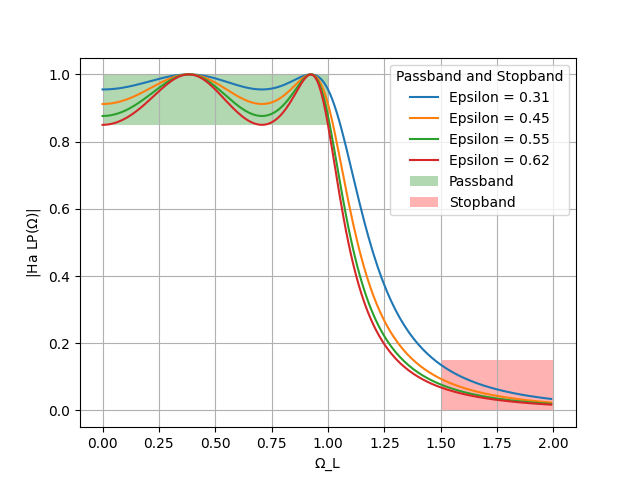
\includegraphics[width=1\columnwidth]{figs/plot1.png}
\caption{The Analog Low-Pass Frequency Response for $0.16  \leq \epsilon \leq 0.62$}
\label{fig:H_for_diff_eb}
\end{figure}

In \figref{fig:H_for_diff_eb} we can observe the equiripple behaviour in passband and monotonic behaviour in stopband. As the value of $\epsilon$ increases the value of $\vert H_{a,LP}(j\Omega_L)\vert$ decreases.\\

\item {The Low Pass Chebyschev Filter:} The next step in design is to find an expression for magnitude response in $s$ domain. 

Using $s=j\Omega$ or in this case $s_{L}=j\Omega_{L}$ we obtain:
\begin{align}
    \vert H_{a,LP}(j\Omega_L)\vert^2 = \frac{1}{1 + \epsilon^2c_N^2(\frac{s_L}{j})}
\end{align}
To find poles equate the denominator to zero:
\begin{align}
    {1 + \epsilon^2c_N^2\brak{\frac{s_L}{j}}} &=0\hspace{5pt }
    \text{where } \hspace{10pt} c_N(x) = cos\brak{Ncos^{-1}\brak{x}} \label{eq:pole_ques}
\end{align}
On solving \eqref{eq:pole_ques} we obtain poles :
\begin{align}
    s_{k} &= -\Omega_{Lp} \sin\brak{A_k}\sinh\brak{B_k} - j\Omega_{Lp}\cos\brak{A_k}\cosh\brak{B_k}
\end{align}
where $k$ is the index of the pole and \\
\begin{align}
    A_k &= \brak{2k+1}\frac{\pi}{2N}\\
    B_k &= \frac{1}{N} \sinh^{-1}\brak{\frac{1}{\epsilon}}
\end{align}
The below code computes the values of $s_k$ and stores it in a text file. 
\begin{lstlisting}
https://github.com/dhanushnayakh03/EE1205/blob/main/Filter_Design/codes/sk_gen.c
\end{lstlisting}
The poles obtained are formulated in the table below.
\begin{table}[H]
    \centering
    
    \resizebox{0.51\textwidth}{!}{
    \begin{tabular}{|c|c|c|}
    \hline
    \textbf{$Pole$} & \textbf{$Value$} \\ \hline
$s[1]$ & $0.1621 - j1.0033$ \\ \hline
$s[2]$ & $0.3913 - j0.4156$ \\ \hline
$s[3]$ & $0.3913 + j0.4156$ \\ \hline
$s[4]$ & $0.1621 + j1.0033$ \\ \hline
$s[5]$ & $-0.1621 - j1.0033$ \\ \hline
$s[6]$ & $-0.3913 - j0.4156$ \\ \hline
$s[7]$ & $-0.3913 + j0.4156$ \\ \hline
$s[8]$ & $-0.1621 + j1.0033$ \\ \hline
    \end{tabular}}
    \caption{Values of $s_k$}
    \label{tab:values poles sk}
    \end{table}


The below code plots the pole-zero plot.
\begin{lstlisting}
https://github.com/dhanushnayakh03/EE1205/blob/main/Filter_Design/codes/plot1.py
\end{lstlisting}
\begin{figure}[H]
\centering
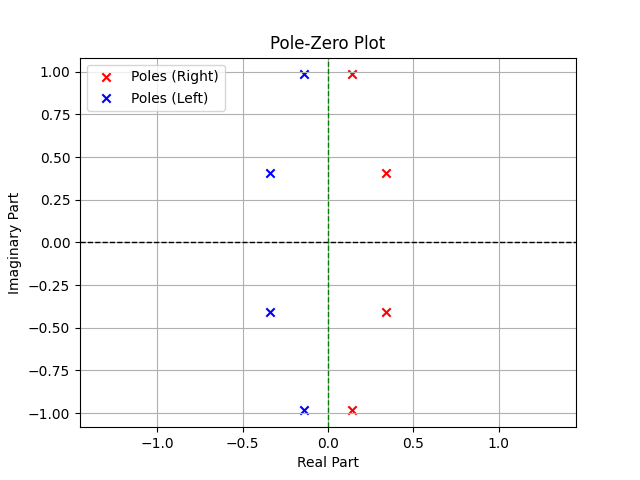
\includegraphics[width=1\columnwidth]{figs/Pole_Zero_plt.png}
\caption{The Pole zero plot and all the poles lie on an ellipse. The left and right poles have been identified as shown.}
\label{fig:pole_zero_plt}
\end{figure}
The poles in the left half of the plane are considered in the design as we intend to design a stable system.\\
Therefore the magnitude response is written as :- 
\begin{align}
    H_{a,LP}(s_L) &= \frac{G_{LP}}{\brak{s_L-s_5}\brak{s_L-s_6}\brak{s_L-s_7}\brak{s_L-s_8}}
\end{align}
where $G_{LP}$ is the gain of the Low pass filter. Refer to \tabref{tab:values poles sk} for $s_k$ values.\\

We know that from \eqref{eq:mag_freq_response}:-
\begin{align}
    \abs{ H_{a,LP}(s_L)} &= \frac{1}{\sqrt{1+\epsilon^2}} \text{at} \hspace{5pt} \Omega_{L}=1 \implies s_{L} = j \label{eq:Gain_eq_LP} 
\end{align}
Substituting respective values in \eqref{eq:Gain_eq_LP} we get $G_{LP}=0.4166$
\begin{align}
     H_{a,LP}(s_L) &= \frac{0.4166}{\brak{s_L-s_5}\brak{s_L-s_6}\brak{s_L-s_7}\brak{s_L-s_8}}\\
     &= \frac{0.4166}{s_{L}^4 + 1.3022s_{L}^3 +1.84781s_{L}^2 + 1.16512s_{L} +0.435003}\label{eq:design}
\end{align}
\end{enumerate}
\end{document}
